\section{IMPLEMENTATION}
\begin{figure*}[thpb]
 \centering
 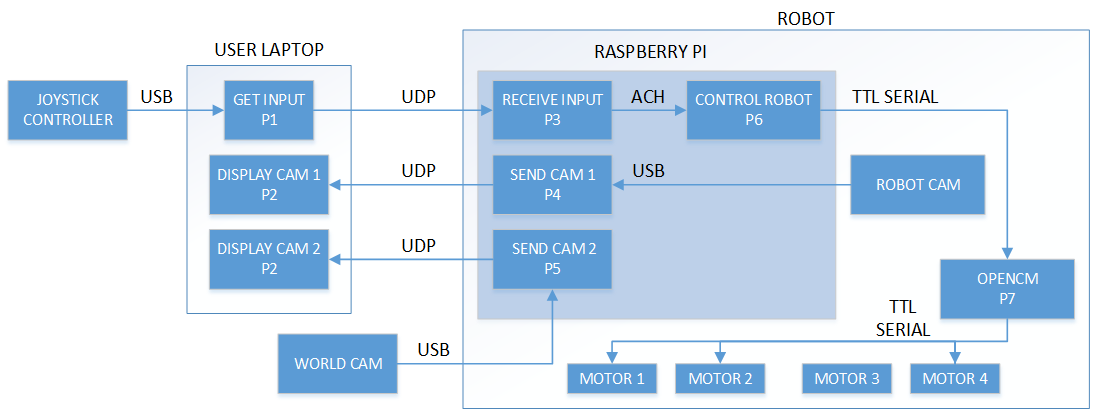
\includegraphics[width=2.0\columnwidth]{./images/cranebot2.png}
  \caption{Crane Robot Communication Diagram}
  \label{fig:cranebot block}
\end{figure*} 

An example implementation of the information gathered is presented here. The objective of this design is to move blocks from an unknown starting location to a goal location. This is to be done remotely under user control with the only visual information coming from the robot. Visual information is collected via two webcams attached to a Raspberry Pi. The Raspberry Pi will receive commands from a remote terminal and control 4 servomotors by sending serial commands to the OpenCM motor controller. To achieve the required teleoperation, user input and both video feeds must be transmitted over a network.

The user will operate the robot with a joystick connected to a laptop. One process runs on the laptop to recieve information from the joystick and transmit to the robot over the network via UDP. UDP was selected for this communication link to ensure the fastest communication to the robot. Low latency was a priority as any lag in commands being received by the robot will proprogate to updating the video feedback and would make teleoperation difficult. Missed messages were of low concern as the frequency of message transmits would be replaced with new commands faster than the user can realize the delay. Command packets can be designed to be two bytes in size to minimize any risk of missed messages.

UDP was also selected for sending both video streams from the robot to be displayed on the user terminal. The video frame information required sending UDP messages at the maximum size limit for a single message. This did increase the probability of a message being missed, but the update rate of the video stream reduced on the impact of missed frames. As the video information is being interpreted by a human and not a computer, lower image resolution and frame rates were acceptable.

In order to have immediate response to user commands, the process collecting data from the joystick needed to operate at a high frequency. This will result in a large amount of messages being transmitted to the Raspberry Pi. Preliminary testing showed that while the user held the joystick down in a certain direction, a large quantites of the same command were stored in the robots UDP buffer. This would cause the robot to continue acting on outdated command information while it processed all received UDP commands. Increasing the update rate of the processes running on the PI to match incomming messages was not an acceptable solution as processing two USB video streams at higher rates was too taxing on the system. This led to errors and corruption of video information.

We needed to utilize the non head of line blocking aspect of the ACH IPC to access the most recent command message at a lower frequency. We incorporated an additional process that would receive UDP message and fill an ACH channel with data. This allowed the command process to update at a rate that matched the video information processed and sent back to the user without overloading the resouces of the Pi. Figure \ref{fig:cranebot block} shows a block diagram of the processes and communication methods for the robot.


By evaluating the conceptual design and objective of this robot, we were able to narrow down the list of potential IPC methods to use. ZMQ would not be a viable candiate for use as the communication delay would be detrimental to the robots operation. There was no need for a complex communication topology as all of the process communication was between a single client/server pair. The Raspberry Pi and the OpenCM modules are single threaded processors and no additional synchronization features of ZMQ would be needed. ROS can be installed on the Pi and would have been possible candidate for use in this system except that the entire system would communicate with TCP at its core. The aforementioned head of line issue with command packets eliminates a sockets based approach for the entire system. Utilzing ACH and ACHD for network communications would allow us to achieve all of our design goals, but would require the user terminal to also have the ACH libraries to be installed. Utilizing sockets for the network communication was essential to build the most flexible system possible and allow for a modular input solution. This led to the combined solution of implemeneting both UDP and ACH for the robot. 
